%-----------------------------------------------%
% Início do plano de aula
%-----------------------------------------------%
\thispagestyle{empty}
\begin{center}
	\begin{minipage}[!]{\linewidth}
        \begin{minipage}[!]{.19\linewidth}
            
\includegraphics[width=\linewidth]{img/logo.png}           
        \end{minipage}
        \begin{minipage}[!]{.8\linewidth}
            \center
            \ABNTEXchapterfont\normalsize\MakeUppercase{\imprimirinstituicao}
            \par
            \vspace*{10pt}                     
            \ABNTEXchapterfont\normalsize\MakeUppercase{\centro}
            \par
            \vspace*{10pt}           
            \ABNTEXchapterfont\normalsize\MakeUppercase{\disciplina}
        \end{minipage}        
    \end{minipage}
    \\ \vspace{0.5cm}
    \rule{\textwidth}{.5pt}   
\end{center}
    \textual
    \begin{center}
      \section{Ondas II}
      \par
    \end{center}
    
    \noindent \textbf{Estagiário(a): }\imprimirautor 
    
    \noindent \textbf{U.E.: }EEB Giovani Pasqualini Faraco
    
    \noindent \textbf{Série: }2º Ano\hfill{}\textbf{Turma: }2º--5
    
    \noindent \textbf{Aula:} 005\hfill{}\textbf{Data:} 04/11/2022\hfill{}\textbf{Duração:} $45\min$
    \rule{\textwidth}{.5pt}
    \bigskip{}  
    

    \noindent
    \begin{center}
      \textbf{O princípio de Huygens}
    \par\end{center}
    \vspace{20pt}
    \noindent \textbf{Resumo da aula:} Com auxílio de simulações computacionais, apresentar o princípio de Huygens como base para a construção do modelo ondulatório para a Luz.
    \smallskip
    \par\noindent \textbf{Habilidades BNCC:} EM13CNT201.
    \medskip
    \subsection*{Objetivo de Aprendizagem}
    \begin{itemize}
        \item Conhecer o princípio de Hyugens e sua importância para a construção de um modelo ondulatório para a luz. 
    \end{itemize}    
    \bigskip{}    
    \noindent \textbf{Núcleo Conceitual:} \emph{Teoria ondulatória da luz; propagação.}
    \newpage
    

    \section*{Procedimento Didático} 
    \noindent\emph{1º Momento:} Problematização Inicial
    \par\noindent\rule{.3\textwidth}{.5pt}  
    \par\noindent\textbf{Tempo previsto:} 10 minutos
    \smallskip
    \par\noindent\textbf{Dinâmica:} Iniciar a aula recapitulando o modelo corpuscular de newton, focar a atenção para uma problemática em que Newton havia estudado, mas não conseguiu tecer alguma explicação utilizando o modelo corpuscular, o fenômeno é a difração.

    Mostrar algumas imagens da difração da Luz, como por exemplo a difração da luz por uma lâmina fina, questioná-los como seria possível, a luz contornar objetos na teoria corpuscular. Abrir a simulação do Phet e executar as simulações da imagem da \autoref{fig:difraction}, explicando detalhadamente o que está ocorrendo 

    \vspace*{10pt}
    \begin{figure}[!ht]        
        \centering              
        \subfloat[\label{fig:difraction-1}]{
            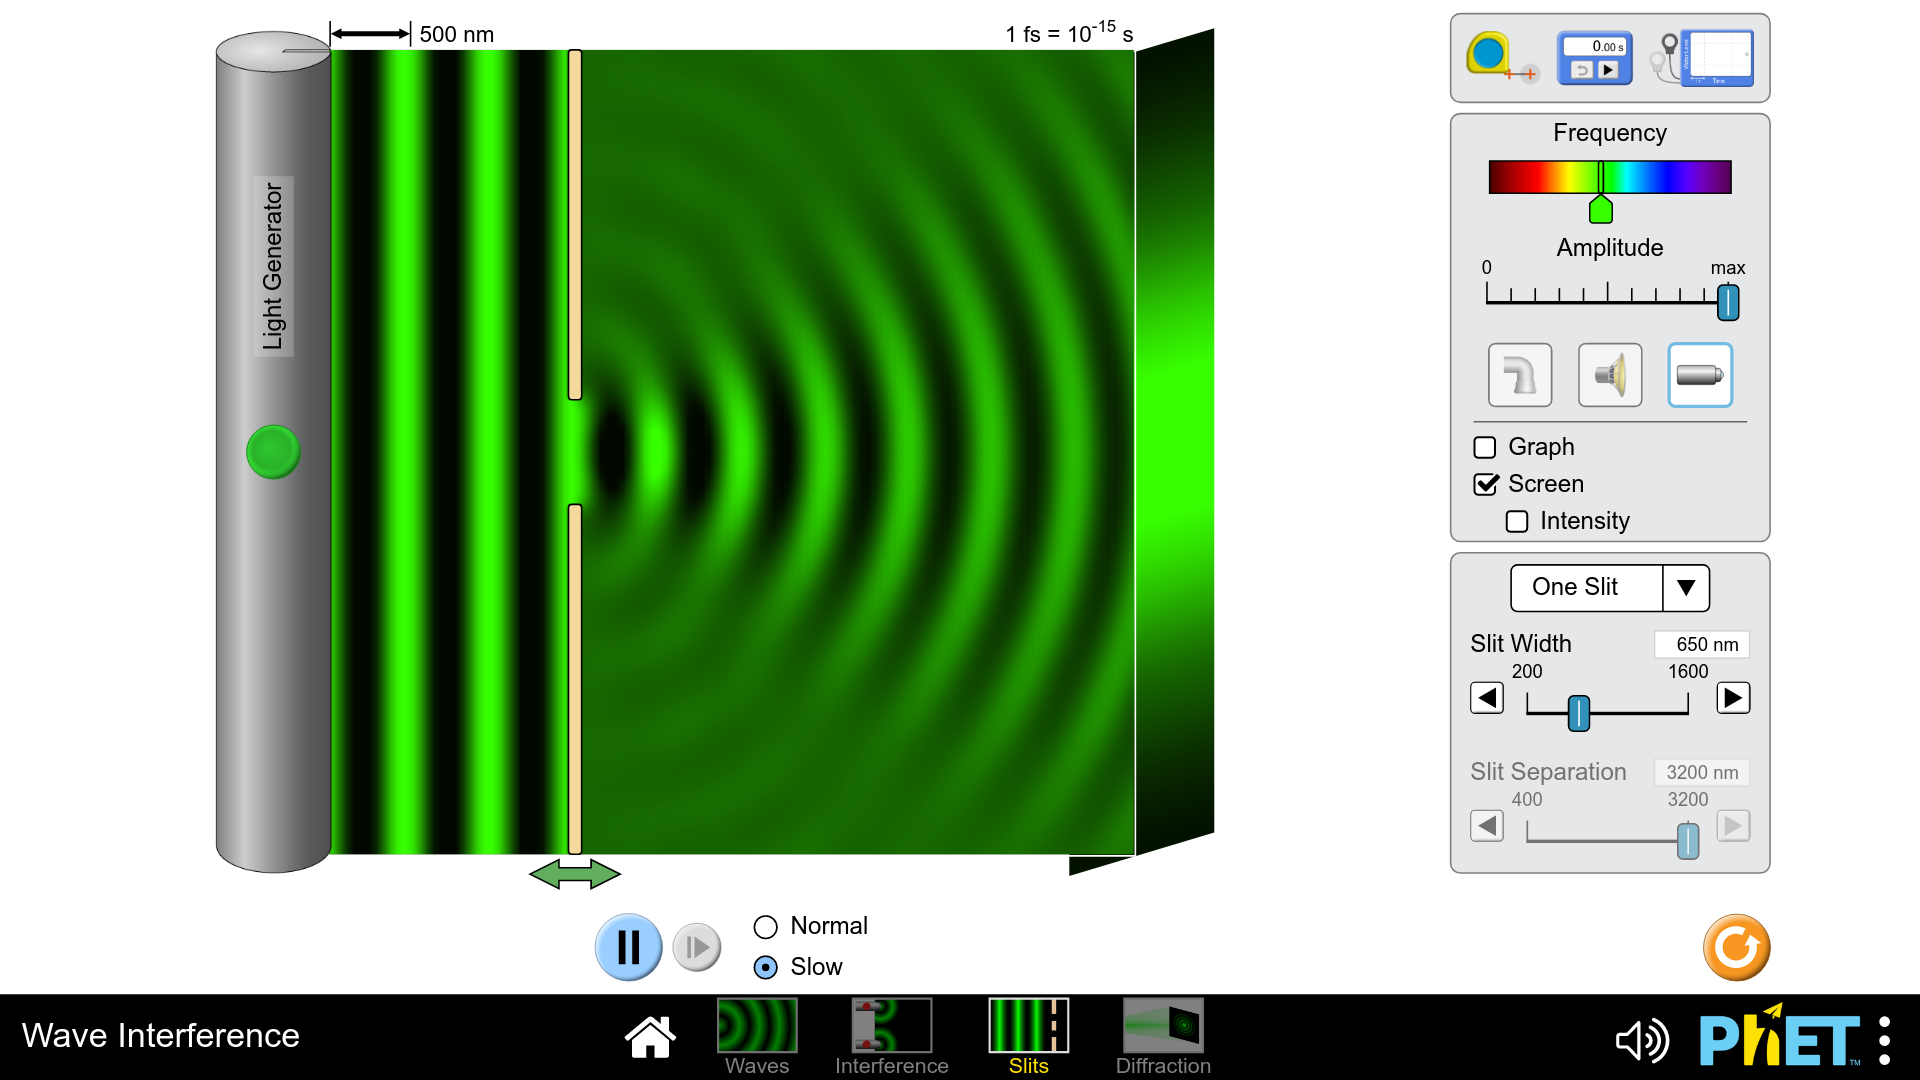
\includegraphics[width=.45\textwidth]{img/difraction-1.png}
        }\hfill
        \subfloat[\label{fig:difraction-2}]{
            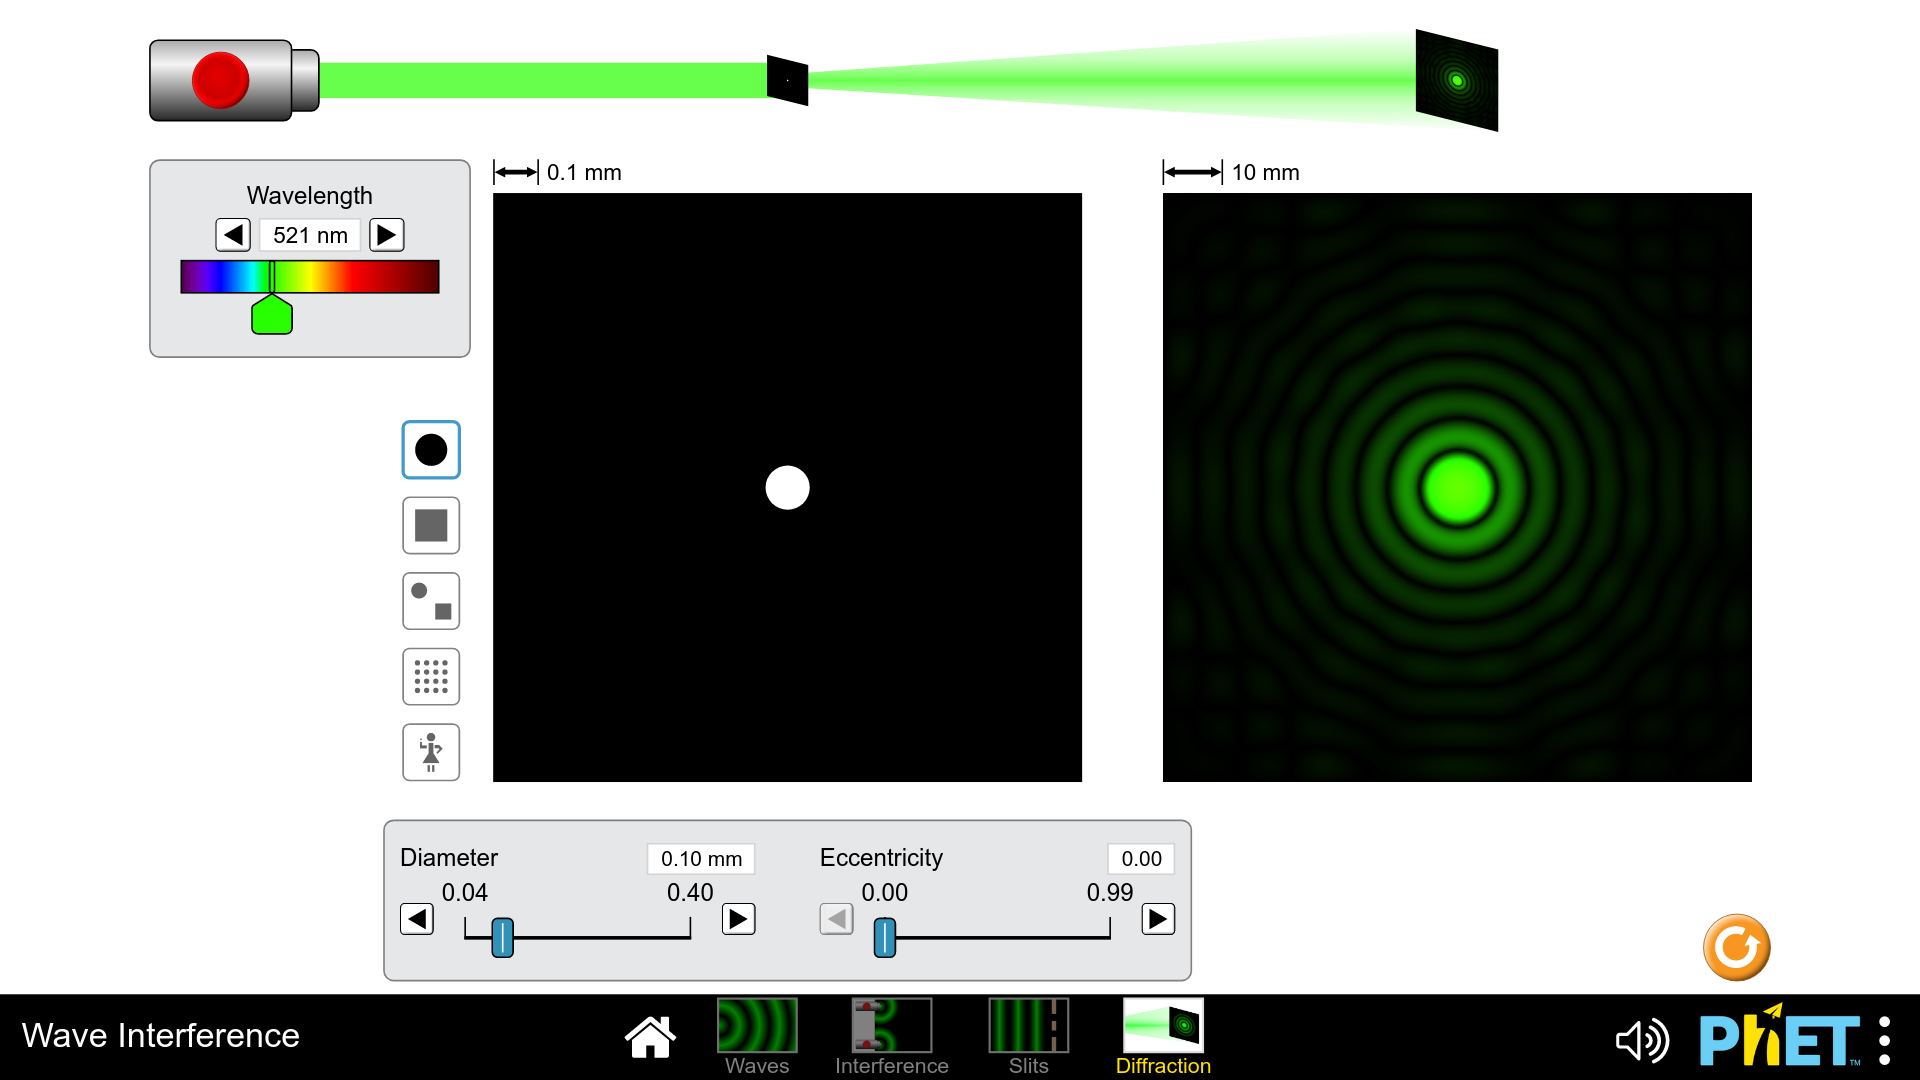
\includegraphics[width=.45\textwidth]{img/difraction-2.png}
        }        
        \caption{Simulação \emph{Phet} em (a), um feixe de ondas planas, passa por um orifício de uma determinada largura, o encurvamento das ondas é visto após o orifício. Em (b), tem-se as figuras de interferência formada num anteparo, ao fazer um feixe de luz atravessar um orifício circular.}
        \label{fig:difraction}
    \end{figure}
    \vspace*{10pt}

    Deixar claro que a simulação faz uso de instrumentos que não existiam à época de Newton e Huygens, mas estes cientistas, conheciam estes fenômenos, inclusive o próprio Newton já havia observado o mesmo fenômeno ocorrendo em lâminas delgadas. Este fenômeno fica bem compreendido por um artifício muito engenhoso estabelecido por Hyugens mo modelo ondulatório, que é o \emph{Princípio de Huygens}
    

% Segundo os autores é nessa etapa que se apresentam questões e/ou situações para discussão com os alunos, visando relacionar o estudo de um conteúdo com situações reais que eles conhecem e presenciam, mas que não conseguem interpretar completa ou corretamente porque provavelmente não dispõem de conhecimentos científicos suficientes. Ou seja, é na problematização que se deseja aguçar explicações contraditórias e localizar as possíveis limitações do conhecimento que vem sendo expressado, quando este é cotejado com o conhecimento científico que já foi selecionado para ser abordado (Delizoicov, Angotti e Pernambuco, 2002, p. 201). Portanto, esse primeiro momento é caracterizado pela compreensão e apreensão da posição dos alunos frente ao tema. É desejável ainda, que a postura do professor se volte mais para questionar e lançar dúvidas sobre o assunto que para responder e fornecer explicações.
    \newpage
    \bigskip{}
    \noindent\emph{2º Momento:} Organização do Conhecimento
    \par\noindent\rule{.3\textwidth}{.5pt}  
    \par\noindent\textbf{Tempo previsto:} 10 minutos
    \smallskip
    \par\noindent\textbf{Dinâmica:} Abrir a \href{https://simphy.com/other-apps/huygen-principle/}{simulação} e iniciar a explicação partindo do caso simples: um ponto gerando uma frente de onda, tal como a \autoref{fig:huygens-1-2}

    \vspace*{10pt}
    \begin{figure}[!ht]        
        \centering              
        \subfloat[\label{fig:huygens-1}]{
            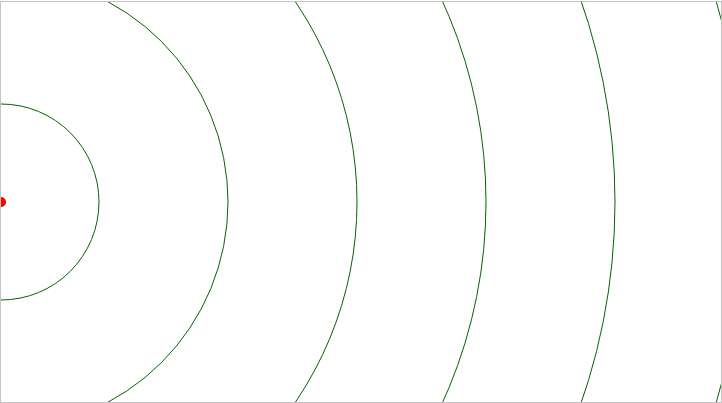
\includegraphics[width=.45\textwidth]{img/principio-huygens-ponto.png}
        }\hfill
        \subfloat[\label{fig:huygens-2}]{
            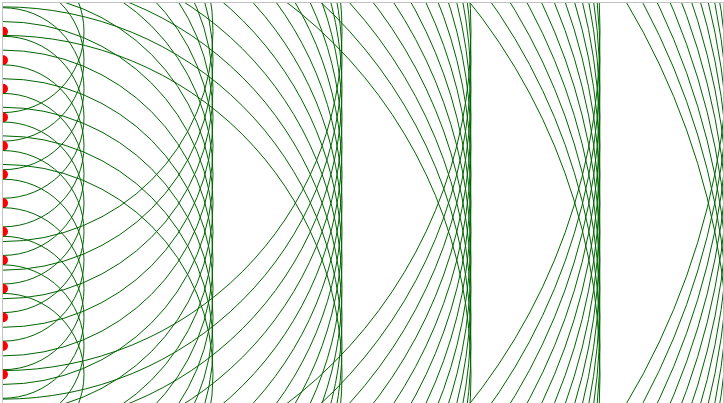
\includegraphics[width=.45\textwidth]{img/principio-huygens-onda-plana.png}
        }        
        \caption{Simulação \emph{Princípio de Huygens} em (a), um ponto simulando um orifício gerador de frentes das frentes de onda. Em (b), vários pontos simulando frentes de ondas planas.}
        \label{fig:huygens-1-2}
    \end{figure}
    \vspace*{10pt}

    Enunciar o princío de Huygens da seguinte maneira:

    \begin{principio}[Huygens]
        Cada ponto de uma frente de onda comporta-se como uma fonte geradora de ondas, que são produzidas com as mesmas características da original.
    \end{principio}

    Por características originais, Huygens quer dizer, mesmo comprimento de onda e mesma frequência.

    Vamos utilizar este princípio para compreender a propagação da luz de passando de um meio para o outro e ver como os fenômenos da reflexão e refração são entendidos no modelo ondulatório.
    

 
    % \begin{figure}[!ht]
    %     \centering
    %     \begin{tikzpicture}[scale=0.8]
        
    %         % define coordinates
    %         \coordinate (O) at (0,0) ;
    %         \coordinate (A) at (0,4) ;
    %         \coordinate (B) at (0,-4) ;
            
    %         % media
    %         \fill[blue!25!,opacity=.3] (-4,0) rectangle (4,4);
    %         \fill[blue!60!,opacity=.3] (-4,0) rectangle (4,-4);
    %         \node[right] at (2,2) {Ar};
    %         \node[left] at (-2,-2) {Água};
        
    %         % axis
    %         \draw[dash pattern=on5pt off3pt] (A) -- (B) ;
        
    %         % rays
    %         \draw[red,ultra thick,reverse directed] (O) -- (130:5.2);
    %         \draw[blue,directed,ultra thick] (O) -- (-70:4.24);
    %         \draw[green,ultra thick,directed] (O) -- (50:5.2);
        
    %         % angles
    %         \draw (0,1) arc (90:130:1);
    %         \draw (0,-1.4) arc (270:290:1.4);
    %         \draw (0,1) arc (90:50:1);
    %         \node[] at (280:1.8)  {$\theta_{2}$};
    %         \node[] at (110:1.4)  {$\theta_{1}$};
    %         \node[] at (70:1.4)   {$\theta_{3}$};
    %     \end{tikzpicture}
    %     \caption{Caption}
    %     \label{fig:my_label}
    % \end{figure}

    % http://hyperphysics.phy-astr.gsu.edu/hbase/phyopt/huygen.html
    % https://simphy.com/other-apps/huygen-principle/
    % https://www.walter-fendt.de/html5/phen/refractionhuygens_en.htm
    

% Delizoicov e Angotti (1990, p. 29) explicam que nesse segundo momento os conhecimentos de Física necessários para a compreensão do tema e da problematização inicial devem ser sistematicamente estudados sob orientação do professor. Definições, conceitos, relações, leis, apresentadas no texto introdutório, serão agora aprofundados. De acordo com Albuquerque, Santos e Ferreira (2015, p. 467) esse é o momento em que os conhecimentos científicos passam a ser incorporados nas discussões. Os alunos começam a desenvolver uma compreensão a respeito da problematização ou situação inicial. Entretanto, para que isso ocorra, materiais devem ser consultados e atividades devem ser sugeridas para complementar as discussões, no sentido de incentivar e melhorar a sistematização dos conhecimentos. Nessa perspectiva, Delizoicov e Angotti (1990) vêm ressaltar a importância de diversificadas atividades, com as quais se poderá trabalhar para organizar a aprendizagem. Sugerem exposições, pelo professor, de definições e propriedades, além de formulações de questões (exercícios de fixação como dos livros didáticos), textos e experiências. Neste sentido, atualmente poderíamos acrescentar as mídias tecnológicas, como televisão, vídeos, filmes, programas tecnológicos, aplicativos de celulares, simulações, entre outros, de modo a auxiliar no processo da sistematização do conhecimento.

    \newpage
    \bigskip
    \noindent\emph{3º Momento:} Aplicação do Conhecimento
    \par\noindent\rule{.3\textwidth}{.5pt}  
    \par\noindent\textbf{Tempo previsto:} 10 minutos
    \smallskip
    \par\noindent\textbf{Dinâmica:} Abrir a próxima \href{https://www.walter-fendt.de/html5/phen/refractionhuygens_en.htm}{simulação}, passar as etapas desta última simulação de forma dialogada. A \autoref{fig:huygens-refracao-reflexao} a seguir mostra as duas situações que devem ser discutidas, para a refração e reflexão.

    
    \vspace*{10pt}
    \begin{figure}[!ht]        
        \centering              
        \subfloat[\label{fig:refracao-ondas}]{
            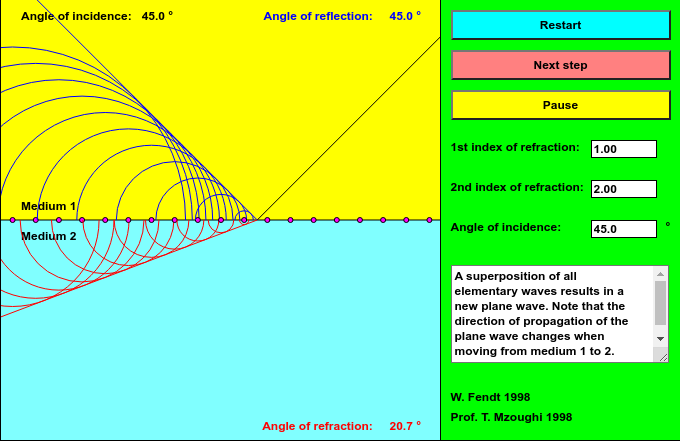
\includegraphics[width=.45\textwidth]{img/refracao-ondas-1.png}
        }\hfill
        \subfloat[\label{fig:reflexao-ondas}]{
            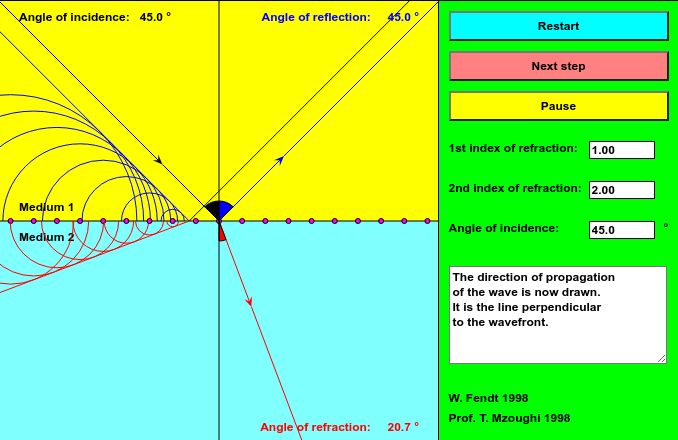
\includegraphics[width=.45\textwidth]{img/reflexao-ondas-1.png}
        }        
        \caption{Simulação \emph{Princípio de Huygens} em (a), uma frente de onda propagando-se do meio menos denso, com ângulo de 45\degree, para um mais denso, alterando a direção de propagação para 20,7\degree. As frentes de onda formadas após a interação com o meio, seguem o princípio de Huygens. Em (b) tem-se destacado as frentes de onda, deslocando-se perpendicularmente com relação a direção de propagação.}
        \label{fig:huygens-refracao-reflexao}
    \end{figure}
    \vspace*{10pt}

    Variar os parâmetros da simulação de forma a deixar claro a incidência perpendicular da frente de onda com relação à velocidade de propagação da mesma. Este fato vai ser importante para deduzir a lei de Snell na próxima aula.

    Por fim, chamar a atenção para a frente de onda refletida pelos pontos sobre a interface, se necessário pausar a simulação no exato momento em que a frente de onda refletida se encontra com o raio refletido traçado na simulação, este fato por si só já demostra lei da reflexão observada na simulação do \emph{PheT}.
    

% Essa última etapa aborda sistematicamente o conhecimento que vem sendo incorporado pelo aluno para analisar e interpretar tanto a situações iniciais que determinaram o seu estudo, como outras situações que não estejam diretamente ligadas ao motivo inicial, mas que são explicadas pelo mesmo conhecimento. (Delizoicov e Angotti, 1990, p. 31). Este é o momento importante para que os alunos encontrem relações entre os temas abordados, não apenas através dos conceitos, mas também de fenômenos que possam ter alguma conexão com as informações apresentadas. No entanto, o professor mantém a postura problematizadora, podendo trazer questionamentos que não foram levantados pelos alunos, como informações e problemas que surgiram do decorrer dos momentos. Além disso, este é um bom momento para o professor formalizar alguns conceitos que não foram aprofundados pelos alunos. (Albuquerque, Santos e Ferreira, 2015).

%-----------------------------------------------%
% FIM do plano de aula
%-----------------------------------------------%